\documentclass[11pt,letterpaper]{article}
\usepackage[lmargin=1in,rmargin=1in,tmargin=1in,bmargin=1in]{geometry}
\usepackage{../style/homework}
\usepackage{../style/commands}
\setbool{quotetype}{true} % True: Side; False: Under
\setbool{hideans}{true} % Student: True; Instructor: False

% -------------------
% Content
% -------------------
\begin{document}

\homework{6: Due 10/02}{Pitter patter, let's get at'er.}{Wayne, Letterkenny}

% Problem 1
\problem{10} For each of the following, describe whether the given dependent variable is a function of the independent variable:
	\begin{enumerate}[(a)]
	\item Independent: the number of days since you purchased your car. \par 
		Dependent: the milage for your car. 
	\item Independent: the number of people in a specific room at noon. \par 
		Dependent: the day of the week.
	\item Independent: the day of the year. \par
		Dependent: the sunrise time. 
	\item Independent: your laptop battery percentage. \par
		Dependent: the time remaining until your laptop runs out of power. 
	\end{enumerate}



\newpage



% Problem 2
\problem{10} Consider the relation plotted below:
	\[
	\fbox{
	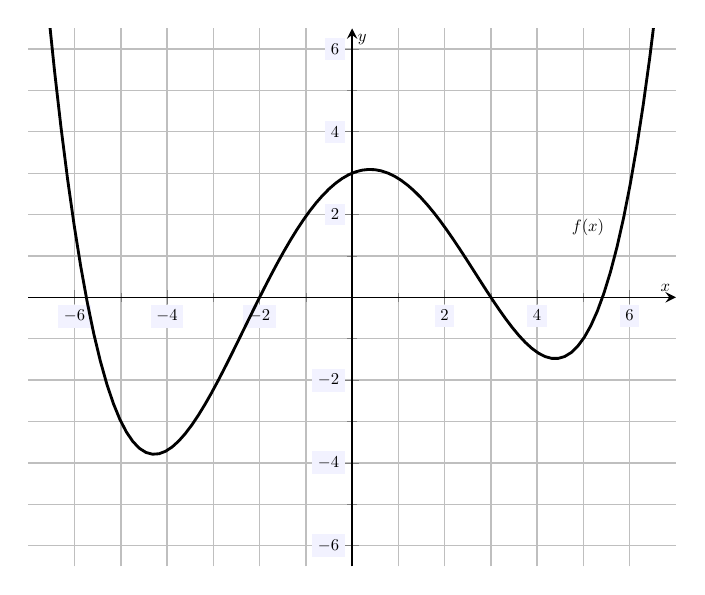
\begin{tikzpicture}[scale=1.2,every node/.style={scale=0.5}]
	\begin{axis}[
	grid=both,
	axis lines=middle,
	ticklabel style={fill=blue!5!white},
	xmin= -7, xmax=7,
	ymin= -6.5, ymax=6.5,
	xtick={-6,-4,-2,0,2,4,6},
	ytick={-6,-4,-2,0,2,4,6},
	minor tick = {-5,-3,...,5},
	xlabel=\(x\),ylabel=\(y\),
	]
	\addplot[domain=-7:7, samples=100,line width=0.03cm] (x,3+0.467857*x-0.601786*x^2-0.0107143*x^3+0.0160714*x^4);
	\node at (5.1,1.7) {$f(x)$};
	\end{axis}
	\end{tikzpicture}
	}
	\]

\begin{enumerate}[(a)]
\item Is the relation, $f(x)$, plotted above a function? Explain. 
\item Find the $y$-intercept.
\item Find the $x$-intercepts. 
\item Find the value of $f(6)$.
\item Find any $x$-values for which $f(x)= 2$.  
\end{enumerate}



\newpage



% Problem 3
\problem{10} Define $f(x)$ to be the relation given by $f(x):= 2.7x + 14.9$.
	\begin{enumerate}[(a)]
	\item Is $f(x)$ a function? Explain.
	\item Find $f(9)$.
	\item Is there an $x_0$ so that $f(x_0)= 20$? If so, find it. If not, explain why. 
	\item Find the $y$-intercept for $f(x)$. 
	\item Find any $x$-intercepts for $f(x)$.
	\end{enumerate}



\newpage



% Problem 4
\problem{10} Let $f(x)$ and $g(x)$ be the functions given by the values in the table below. \par
	\begin{table}[H]
	\centering
	\begin{tabular}{r||rrrrr}
	$x$ & $-2$ & $-1$ & $0$ & $1$ & $2$ \\ \hline
	$f(x)$ & $4$ & $5$ & $-1$ & $6$ & $0$ \\
	$g(x)$ & $3$ & $-2$ & $7$ & $0$ & $-1$
	\end{tabular}
	\end{table} \par
Compute the following:
	\begin{enumerate}[(a)]
	\item $f(-2) - g(1)$ 
	\item $(f + g)(0)$
	\item $(fg)(-1)$
	\item $(f \circ g)(2)$
	\item $(g \circ f)(2)$
	\end{enumerate}


\end{document}